\documentclass[tikz]{standalone}

\usepackage[outline]{contour}
\usepackage{mathabx}
%\usepackage{tikz}

% tikz setup
\usetikzlibrary{automata, positioning, arrows}

\contourlength{0.5pt}


\tikzstyle{every path} = [draw=black]
\tikzstyle{every state} = [fill=white]

\tikzset{%
    ->,
    >=stealth',
    node distance=2cm,
    initial text=$ $,
}

\newcommand{\nodestroke}[1]{\contour{white}{#1}}

\begin{document}
    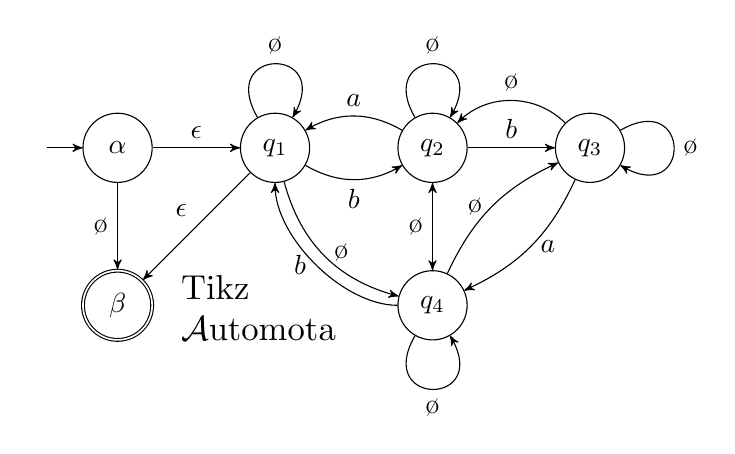
\begin{tikzpicture}

        % nodes
        \node[state] (q1) {$q_1$};
        \node[state, right of=q1] (q2) {$q_2$};
        \node[state, right of=q2] (q3) {$q_3$};
        \node[state, below of=q2] (q4) {$q_4$};
        \node[state, initial, left of=q1] (qA) {$\alpha$};
        \node[state, accepting, below of=qA] (qB) {$\beta$};

        % text node
        \node [right of=qB, align=left, xshift=-6px, yshift=-1px, scale=1.25] (text) {Tikz$\righttoleftarrow$\\$\mathcal{A}$utomota};

        \draw (q1) edge[below, bend right] node{\nodestroke{$b$}} (q2)
        (q2) edge[above, bend right] node{\nodestroke{$a$}} (q1)
        (q2) edge[above] node{\nodestroke{$b$}} (q3)
        (q3) edge[right, bend left=20] node{\nodestroke{$a$}} (q4)
        (q4) edge[left, bend left=45, looseness=0.8] node{\nodestroke{$b$}} (q1)

        % null transitions
        (q1) edge[right, bend right] node[yshift=1px]{\nodestroke{\o}} (q4)
        (q2) edge[<->, left] node{\nodestroke{\o}} (q4)
        (q4) edge[left, bend left=20] node{\nodestroke{\o}} (q3)
        (q3) edge[bend right=45, above] node{\nodestroke{\o}} (q2)
        (qA) edge[above] node{\nodestroke{$\epsilon$}} (q1)
        (q1) edge[above left] node{\nodestroke{$\epsilon$}} (qB)
        (qA) edge[left] node{\nodestroke{\o}} (qB)
        (q1) edge[loop above, in=60, out=120, looseness=6] node{\nodestroke{\o}} (q1)
        (q2) edge[loop above, in=60, out=120, looseness=6] node{\nodestroke{\o}} (q2)
        (q3) edge[loop right, in=-30, out=30, looseness=6] node{\nodestroke{\o}} (q3)
        (q4) edge[loop below, in=-60, out=-120, looseness=6] node{\nodestroke{\o}} (q4)
        ;

    \end{tikzpicture}
\end{document}